\section{The Proposed Algorithm}\label{sec:algorithm}

It was shown in \sectionname~\ref{sec:chromatic} that the Christofides algorithm with the Wang improvements
outperforms the Zykov algorithm.  But can some additional bounding conditions be added to the Zykov algorithm to
close the performance gap?  This section proposes a new Zykov-like algorithm that attempts to do just that.  An
early version of this new algorithm was first introduced by the author and his advisor in collaboration with a team
of mechanical engineering researchers from SUNY Buffalo \cite{cavallaro}.

The major advantages of the Christofides and the Zykov algorithms are that they don't depend on the connectedness
of a graph, an example of a chromatic coloring is readily available, and the fact that the algorithms can be coded
rather easily to run on a computer.  Their major disadvantage is their high runtime complexity, which is inherent
to the chromatic number problem.

Thus, the goals of the proposed algorithm are as follows:
\begin{enumerate}
\item It should not depend on whether the graph is connected or not.
\item An example of a chromatic coloring should be readily available.
\item It can be easily coded for execution on a computer.
\item It has better runtime performance than the well-known algorithms over the target range of less than
  \(20\) nodes with less than \(50\%\) edge density.
\end{enumerate}

To accomplish these goals, the proposed algorithm loops on successively higher values of \(k\).  For each candidate
\(k\) value, a graph \(G\) is assumed to be \colorable{k} and a modified version of a Zykov algorithm is executed
on \(G\) to either prove or disprove this assumption.  Since a candidate \(k\) value is known, certain reversible
steps can be applied to mutate \(G\) into simpler graphs with equivalent colorability and test for early
termination of the Zykov tree.  The first \(k\) for which \(G\) (or one of its simplifications) is found to be
\colorable{k} is the chromatic number of \(G\).

One slight disadvantage of the proposed algorithm is that whereas the other algorithms readily provide examples of
actual chromatic colorings, the proposed algorithm requires an additional step to construct a chromatic coloring: a
greedy algorithm with a particular sorting of the vertices.  The coloring step is discussed in detail in
\sectionname~\ref{sec:sub:sub:coloring}.  Albeit additional work, this extra coloring step is P-time so it does
not have a significant impact on the performance of the proposed algorithm.

The proposed algorithm accepts a graph \(G\) as input and provides \(\X(G)\) and a chromatic coloring as output and
is composed of the following components:
\begin{enumerate}
\item A main routine that loops on increasing values of \(k\).
\item The Bron Kerbosch algorithm used by the main routine to determine a lower bound \(k_{min}\) for the chromatic
  number of \(G\).
\item The last-first with color interchange greedy coloring algorithm used by the main routine to determine an
  upper bound \(k_{max}\) for the chromatic number of \(G\) and a corresponding \coloring{k_{max}} of \(G\).
\item A recursive subroutine that runs a modified Zykov algorithm with additional pruning to determine if
  \(G\) is \colorable{k}.
\item The Edwards Elphick algorithm used by the recursive subroutine to determine a lower bound for the chromatic
  number of a graph.
\item A coloring routine called by the main routine to construct a chromatic coloring of \(G\) based on the results
  of the algorithm.
\end{enumerate}

The main routine, recursive subroutine, and coloring routine are summarized in the following sections.  A complete
description of the theorems that support the various steps in the algorithm and the application of the algorithm to
a sample graph then follow.

\subsection{The Main Routine}\label{sec:sub:main}

The main routine accepts a graph \(G\) as input and returns \(\X(G)\) and a chromatic coloring for \(G\).  It
initially computes a chromatic number lower bound using Bron Kerbosch and a chromatic number upper bound using
greedy last-first with color interchange.  The latter also provides a default coloring.  If the lower and upper
bounds match then the default coloring is accepted.  If not, then the main routine loops on increasing values of
\(k\), starting with the lower bound and going no further than the upper bound.  For each value of \(k\), the
recursive subroutine is called to execute a modified Zykov algorithm in order to determine if \(G\) is
\colorable{k}.  If \(k\) reaches the upper bound then the default coloring is accepted as chromatic.

Instead of walking a single Zykov tree for the whole graph \(G\), the Wang technique is used to mutate \(G\) into
smaller graphs \(G_i\) by selecting a vertex that occurs in the least number of MISs in \(G\).  Each of these MISs
implies a set of vertex contractions and edge additions that are applied to \(G\) to construct the corresponding
\(G_i\).  Thus, the modified Zykov algorithm is applied in sequence to these separate \(G_i\) for each \(k\) value.
The first successful return identifies \(\X(G)\) and then the coloring routine is called to construct the final
coloring based on the information from the successful tree.

The steps of the main routine are as follows:

\begin{enumerate}
\item\label{step:outer:bron} Use the Bron Kerbosch algorithm to compute a chromatic lower bound \(k_{min}\)
  for the input \(G\).

\item\label{step:outer:greedy} Use the greedy last-first with color interchange algorithm to compute a chromatic
  number upper bound \(k_{max}\) and a default \coloring{k_{max}} for \(G\).

\item\label{step:outer:initk} Initialize \(k\) to \(k_{min}\).

\item\label{step:outer:match} If \(k_{min}=k_{max}\) then accept the default coloring found in
  step~\ref{step:outer:greedy} and go to step~\ref{step:outer:done}.

\item\label{step:outer:trees} Use the Bron algorithm on \(\bar{G}\) to find all the MISs in \(G\).  Select a vertex
  that occurs in the smallest number of MISs and then use those MISs to construct \(n\) graphs that are the roots
  of \(n\) Zykov trees.  Each tree is constructed from \(G\) by contracting the vertices in the MIS and adding
  edges between the contracted vertex and all vertices not in the MIS.  Each tree is also associated with an
  initially empty list of removed vertices \(S\).

\item\label{step:outer:check} If \(k=k_{max}\) then accept the default coloring found in
  step~\ref{step:outer:greedy} and go to step~\ref{step:outer:done}.

\item\label{step:outer:call} Call the recursive subroutine on each tree to determine if its \(G\) is \colorable{k}.
  The recursive subroutine accepts the current tree's graph \(G\) and removed vertex list \(S\) as input and
  returns a Boolean result \(R\).  The called routine may simplify \(G\) and may append removed vertices to
  \(S\).  If a tree results in a solution (\(R=\)true) then go to step~\ref{step:outer:color}.

\item\label{step:outer:incrk} Increment \(k\) and go to step~\ref{step:outer:check}.

\item\label{step:outer:color} Call the coloring routine to construct the final coloring based on the successful
  tree's final state of \(G\) and \(S\).

\item\label{step:outer:done} Return the current \(k\) as the chromatic number and the found chromatic coloring.
\end{enumerate}

A flowchart of these steps is shown in \figurename~\ref{fig:outer}.

\begin{figure}[H]
  \centering
  \scalebox{0.75}{
    \begin{tikzpicture}[>=latex']
      \node (start) [draw,terminal] at (0,0) {START};
      \node (bron) [draw,predproc,below=of start]
            {\(\begin{array}{c} \text{BRON}\ G \\ \text{GREEDY}\ G \end{array}\)};
      \node (kinit) [draw,process,below=of bron] {\(k=k_{min}\)};
      \node (kcheck) [draw,decision,below=of kinit] {\(k_{min}=k_{max}\)?};
      \node (trees) [draw,predproc,below=of kcheck] {TREES \(G\)};
      \node (kcheck2) [draw,decision,below=of trees] {\(k=k_{max}\)?};
      \node (cdef) [draw,process,left=2cm of kcheck2] {\(c=c_{def}\)};
      \node (done) [draw,terminal,below=of cdef] {RETURN \(k,c\)};
      \node (iinit) [draw,process,below=of kcheck2] {\(i=1\)};
      \node (icheck) [draw,decision,below=of iinit] {\(i\le n\)?};
      \node (kinc) [draw,process,right=2cm of icheck] {\(k=k+1\)};
      \node (select) [draw,process,below=of icheck] {\(\begin{array}{c} G=G[i] \\ S=S[i] \end{array}\)};
      \node (zykov) [draw,predproc,below=of select] {ZYKOV \(G,S,k\)};
      \node (check) [draw,decision,below=of zykov] {\(R\)?};
      \node (iinc) [draw,process,below=of check] {\(i=i+1\)};
      \node (color) [draw,predproc,right=2cm of check] {COLOR \(G,S\)};
      \node (done2) [draw,terminal,below=of color] {RETURN \(k,c\)};
      \draw [->] (start) -- node [auto] {\(G\)} (bron);
      \draw [->] (bron) -- node [auto] {\(k_{min},k_{max},c_{def}\)} (kinit);
      \draw [->] (kinit) -- (kcheck);
      \draw [->] (kcheck) -- node [auto] {NO} (trees);
      \draw [->] (trees) -- node [auto] {\(G[1:n],S[1:n]\)} (kcheck2);
      \draw [->] (kcheck2) -- node [auto,swap] {YES} (cdef);
      \draw [->] (kcheck) -| node [auto,swap,pos=0.2] {YES} (cdef);
      \draw [->] (cdef) -- (done);
      \draw [->] (kcheck2) -- node [auto] {NO} (iinit);
      \draw [->] (iinit) -- (icheck);
      \draw [->] (icheck) -- node [auto] {NO} (kinc);
      \draw [->] (kinc) |- (kcheck2);
      \draw [->] (icheck) -- node [auto] {YES} (select);
      \draw [->] (select) -- (zykov);
      \draw [->] (zykov) -- node [auto] {\(G,S,R\)} (check);
      \draw [->] (check) -- node [auto] {NO} (iinc);
      \draw [->] (iinc) -- ++(-3cm,0) |- (icheck);
      \draw [->] (check) -- node [auto] {YES} (color);
      \draw [->] (color) -- node [auto] {\(c\)} (done2);
    \end{tikzpicture}
  }
  \caption{The proposed algorithm main routine.}
  \label{fig:outer}
\end{figure}

Note that in the case of the null or an empty graph, the upper and lower bounds for \(k\) will match and the main
routine will terminate immediately with the default greedy coloring.  Thus, the recursive subroutine is always
called with \(k\ge2\).  Also note that the main routine is guaranteed to terminate because \(k\) will eventually
reach \(k_{max}\) or the recursive subroutine will return true when a simplification occurs such that \(n(G)\le k\).

\subsection{The Recursive Subroutine}\label{sec:sub:called}

The recursive subroutine executes a modified version of a Zykov algorithm that determines whether a graph is
\colorable{k}.  It accepts the current state of \(G\) of order \(n\) and size \(m\) and the current value of
\(k\ge2\) as inputs.  It returns a possibly simplified version of \(G\) and a boolean value indicating whether or
not \(G\) is \colorable{k}.  Internally, various tests are applied to prune the corresponding Zykov tree or abandon
it all together based on the current value of \(k\).

The steps of the recursive subroutine and references to their associated theorems are as follows:

\begin{enumerate}
\item\label{step:sub:sinit} Initialize \(S'\) to the emptyset.

\item\label{step:sub:check} If \(n\le k\) then go to step~\ref{step:sub:success} (\theoremname~\ref{thm:nlek}).

\item\label{step:sub:dencalc} Calculate a maximum edge threshold:
  \[a=\frac{n^2(k-1)}{2k}\]

\item\label{step:sub:density} If \(m>a\) then return false (Corollary~\ref{cor:density}).

\item\label{step:sub:smallcalc} Construct the set \(X\) of all vertices with degree less than \(k\):
  \[X=\setb{v\in V(G)}{\deg(v)<k}\]

\item\label{step:sub:small} If \(X\ne\emptyset\) then append \(X\) to \(S'\), replace \(G\) with \(G-X\), and go to
  step~\ref{step:sub:check} (Corollary~\ref{cor:lowdeg}).

\item\label{step:sub:kadj} If \(n<k_{adj}\) then \(k_{adj}=n\).

\item\label{step:sub:lower} Use the Edwards Elphick algorithm to calculate a new lower bound \(\ell\) for \(G\).

\item\label{step:sub:bound} If \(\ell\ge k_{adj}\) then return false.

\item\label{step:sub:common} Calculate the common number of neighbors between each pair of vertices in \(G\),
  stopping if one vertex's neighborhood is found to be a subset of another.

\item\label{step:sub:subset} If \(G\) has vertices \(u\) and \(v\) such that \(N(u)\subseteq N(v)\) then replace
  \(G\) with \(G\cdot uv\) and go to step~\ref{step:sub:check} (Theorem~\ref{thm:subset}).

\item\label{step:sub:select} Let \(b\) be the smallest number of common neighbors between any pair of vertices in
  \(G\) as found in step~\ref{step:sub:common}:
  \[b=\min_{u,v\in V(G)}\abs{N(u)\cap N(v)}\]

\item\label{step:sub:ubcalc} Calculate an upper bound for the minimum number of common neighbors between any pair
  of vertices in \(G\):
  \[c=n-2-\frac{n-2}{k-1}\]

\item\label{step:sub:ubcheck} If \(b>c\) then return false (Corollary~\ref{cor:inter}).

\item\label{step:sub:select2} Select two non-adjacent vertices \(u,v\in V(G)\) with the smallest number of common
  neighbors as found in step~\ref{step:sub:common}.  It will be shown below that such a pair of vertices is
  guaranteed to exist in the current state of \(G\).

\item\label{step:sub:call1} Assume that \(u\) and \(v\) are assigned the same color by letting \(G'=G\cdot uv\) and
  recursively calling this routine to see if \(G'\) is \colorable{k}.

\item\label{step:sub:result1} If \(G'\) is \colorable{k} then replace \(G\) with \(G'\) and go to
  step~\ref{step:sub:success} (Theorem~\ref{thm:recurse}).

\item\label{step:sub:call2} Assume that \(u\) and \(v\) are assigned different colors by letting \(G'=G+uv\) and
  recursively calling this subroutine to see if \(G'\) is \colorable{k}.

\item\label{step:sub:result1} If \(G'\) is \colorable{k} then replace \(G\) with \(G'\) and go to
  step~\ref{step:sub:success} (Theorem~\ref{thm:recurse}).

\item\label{step:sub:fail} Since neither of the assumptions in steps \ref{step:sub:call1} nor \ref{step:sub:call2}
  hold, conclude that \(G\) is not \colorable{k} and return false.

\item\label{step:sub:success} Replace \(S\) with \(S'\) and return true.
\end{enumerate}

A flowchart of these steps is shown in \figurename~\ref{fig:called}.

\begin{figure}[H]
  \centering
  \scalebox{0.55}{
    \begin{tikzpicture}[>=latex']
      \node (start) [draw,terminal] at (0,0) {START};
      \node (kcheck) [draw,decision,below=of start] {\(n\le k\)?};
      \node (rtrue1) [draw,process,right=2cm of kcheck] {\(R=\)TRUE};
      \node (return1) [draw,terminal,below=of rtrue1] {RETURN \(R,G,S\)};
      \node (ecalc) [draw,process,below=of kcheck] {\(a=\frac{n^2(k-1)}{2k}\)};
      \node (echeck) [draw,decision,below=of ecalc] {\(m\le a\)?};
      \node (xcalc) [draw,process,below=of echeck] {\(X=\setb{v\in V(G)}{\deg(v)<k}\)};
      \node (xcheck) [draw,decision,below=of xcalc] {\(X=\emptyset\)?};
      \node (remnode) [draw,process,left=of xcheck] {\(\begin{array}{c} G=G-X \\ S=S+X \end{array}\)};
      \node (xjoin) [coordinate] at ($(remnode)-(2cm,0)$) {};
      \node (common) [draw,process,below=of xcheck] {\(\abs{N(u)\cap N(v)}\)};
      \node (subcheck) [draw,decision,below=of common] {\(N(u)\subseteq N(v)\)?};
      \node (subcon) [draw,process,left=of subcheck] {\(G=G\cdot uv\)};
      \node (mincom) [draw,process,below=of subcheck] {\(b=\min\abs{N(u)\cap N(v)}\)};
      \node (mincalc) [draw,process,below=of mincom] {\(c=n-2-\frac{n-2}{k-1}\)};
      \node (mincheck) [draw,decision,below=of mincalc] {\(b\le c\)?};
      \node (mjoin) [coordinate] at ($(mincheck)+(4cm,0)$) {};
      \node (lbcalc) [draw,predproc,below=of mincheck] {EDWARDS \(G\)};
      \node (lbcheck) [draw,decision,below=of lbcalc] {\(\ell\le k\)?};
      \node (rfalse1) [draw,process,right=2cm of lbcheck] {\(R=\)FALSE};
      \node (return2) [draw, terminal,below=of rfalse1] {RETURN \(R,G,S\)};
      \node (save1) [draw,process,right=6cm of rtrue1] {\(\begin{array}{c} G'=G\cdot uv \\ S'=S \end{array}\)};
      \node (call1) [draw,predproc,below=of save1] {CALL \(G',S',k\)};
      \node (check1) [draw,decision,below=of call1] {\(R\)?};
      \node (save2) [draw,process,below=of check1] {\(\begin{array}{c} G'=G+uv \\ S'=S \end{array}\)};
      \node (call2) [draw,predproc,below=of save2] {CALL \(G',S',k\)};
      \node (check2) [draw,decision,below=of call2] {\(R\)?};
      \node (return3) [draw,terminal,below=of check2] {RETURN \(R,G,S\)};
      \node (update) [draw,process,right=3cm of check2] {\(\begin{array}{c} G=G' \\ S=S' \end{array}\)};
      \draw [->] (start) -- node [auto] {\(G,S,k\)} (kcheck);
      \draw [->] (kcheck) -- node [auto,pos=0.2] {YES} (rtrue1);
      \draw [->] (rtrue1) -- (return1);
      \draw [->] (kcheck) -- node [auto] {NO} (ecalc);
      \draw [->] (ecalc) -- (echeck);
      \draw [->] (echeck) -- node [auto] {YES} (xcalc);
      \draw [->] (xcalc) -- (xcheck);
      \draw [->] (xcheck) -- node [auto,swap] {NO} (remnode) -- (xjoin);
      \draw [->] (xcheck) -- node [auto] {YES} (common);
      \draw [->] (common) -- (subcheck);
      \draw [->] (subcheck) -- node [auto,swap] {YES} (subcon);
      \draw [->] (subcon) -| (xjoin) |- (kcheck);
      \draw [->] (subcheck) -- node [auto] {NO} (mincom);
      \draw [->] (mincom) -- (mincalc);
      \draw [->] (mincalc) -- (mincheck);
      \draw [->] (mincheck) -- node [auto] {YES} (lbcalc);
      \draw [->] (mincheck) -- node [auto,pos=0.2] {NO} (mjoin);
      \draw [->] (lbcalc) -- node [auto] {\(\ell\)} (lbcheck);
      \draw [->] (lbcheck) -- node [auto,pos=0.2] {NO} (rfalse1);
      \draw [->] (echeck) -| node [auto,pos=0.1] {NO} (mjoin) -- (rfalse1);
      \draw [->] (rfalse1) -- (return2);
      \draw [->] (lbcheck) -- node [auto,pos=0.2] {YES} ++(0,-3cm) -- ++(8cm,0) |- (save1);
      \draw [->] (save1) -- (call1);
      \draw [->] (call1) -- node [auto] {\(R,G',S'\)} (check1);
      \draw [->] (check1) -- node [auto] {NO} (save2);
      \draw [->] (save2) -- (call2);
      \draw [->] (call2) -- node [auto] {\(R,G',S'\)} (check2);
      \draw [->] (check2) -- node [auto] {NO} (return3);
      \draw [->] (check2) -- node [auto,pos=0.2] {YES} (update);
      \draw [->] (check1) -| node [auto,pos=0.1] {YES} (update);
      \draw [->] (update) |- (return3);
    \end{tikzpicture}
  }
  \caption{The proposed algorithm recursive subroutine.}
  \label{fig:called}
\end{figure}

Step~\ref{step:sub:check} is the success termination condition.  Success occurs when \(G\) is simplified by
removing sufficent vertices (steps~\ref{step:sub:smallcalc}--\ref{step:sub:subset}) and the main routine has
sufficiently incremented \(k\) (step~\ref{step:outer:incrk}) such that \(n\le k\).

Steps~\ref{step:sub:smallcalc}--\ref{step:sub:subset} attempt to remove vertices to achieve a simpler graph that is
equivalently \colorable{k}.  Each time a vertex is removed, the Zykov branches associated with that vertex are
pruned.  Since these same steps would just be repeated for \(k+1\), the subroutine returns the current state of the
possibly simplified \(G\) to the main routine as a starting point for the next candidate value of \(k\).

Steps~\ref{step:sub:dencalc}--\ref{step:sub:density} and \ref{step:sub:select}--\ref{step:sub:ubcheck} apply tests
that attempt to disprove that the current state of \(G\) is \colorable{k} for the current value of \(k\).  If so,
then the current Zykov tree is abandoned and the subroutine returns false.  This allows the main routine to continue
with \(k+1\).

The remaining steps of the recursive subroutine, steps~\ref{step:sub:select2}--\ref{step:sub:fail}, constitute the
recursive portion of the modified Zykov algorithm.  The recursive calls are guaranteed to terminate because either
there will be sufficient vertex contractions such that \(n\le k\), resulting in a true return, or sufficient edge
additions such that the graph becomes complete and (as will be shown) is rejected by step~\ref{step:sub:density},
resulting in a false return.  Note that in the event of a false return, any modifications to the current state of
\(G\) resulting from the recursive calls are not returned to the main routine.

\subsubsection{The Coloring Routine}\label{sec:sub:sub:coloring}

\subsection{Supporting Theorems}\label{sec:sub:theorems}

This section contains the theorems that support the steps in the recursive subroutine.  Remember that the success
check of step~\ref{step:sub:check} is already supported by \theoremname~\ref{thm:nlek}.

\subsubsection{Maximum Edge Threshold}\label{sec:sub:sub:edges}

The maximum edge threshold test of steps~\ref{step:sub:dencalc} and \ref{step:sub:density} is supported by
Theorem~\ref{thm:density}.

\begin{theorem}[Maximum Edge Threshold]
  \label{thm:density}
  Let \(G\) be a graph of order \(n\) and size \(m\) and let \(k\in\N\).  If \(G\) is \colorable{k} then:
  \[m\le\frac{n^2(k-1)}{2k}\]
\end{theorem}

\begin{proof}
  Assume that \(G\) is \colorable{k}.  This means that \(V(G)\) can be distributed into \(k\) independent (some
  possibly empty) subsets.  Call these subsets \(A_1,\ldots A_k\) and let \(a_i=\abs*{A_i}\).  Thus, each \(v\in
  A_i\) can be adjacent to at most \(n-a_i\) other vertices in \(G\), and hence the maximum number of edges
  incident to vertices in \(A_i\) is given by: \(a_i(n-a_i)=na_i-a_i^2\).  Now, using Theorem~\ref{thm:first}, the
  maximum number of edges in \(G\) is given by:
  \[m\le\frac{1}{2}\sum_{i=1}^k(na_i-a_i^2)\]
  with the constraint:
  \[\sum_{i=1}^ka_i=n\]
  This problem can be solved using the Lagrange multiplier technique.  We start by defining:
  \begin{align*}
    F(a_1,\ldots,a_k) &= f(a_1,\ldots,a_k)-\l g(a_1,\ldots,a_k) \\
    &= \frac{1}{2}\sum_{i=1}^k(na_i-a_i^2)-\l\sum_{i=1}^ka_i \\
    &= \sum_{i=1}^k\left(\frac{1}{2}na_i-\frac{1}{2}a_i^2-\l a_i\right)
  \end{align*}
  Now, optimize by taking the gradient and setting the resulting vector equation equal to the zero vector:
  \[\vec{\nabla}F=\sum_{i=1}^k(\frac{n}{2}-a_i-\l)\hat{a_i}=\vec{0}\]
  This results in a system of \(k\) equations of the form:
  \[\frac{n}{2}-a_i-\l=0\]
  And so:
  \[a_i=\frac{n}{2}-\l\]
  Plugging this result back into the contraint:
  \[\sum_{i=1}^ka_i=\sum_{i=1}^k\left(\frac{n}{2}-\l\right)=k\left(\frac{n}{2}-\l\right)=n\]
  Solving for \(\l\) yields:
  \[\l=\frac{n}{2}-\frac{n}{k}\]
  And finally, to get \(a_i\) in terms of \(n\) and \(k\):
  \[a_i=\frac{n}{2}-\left(\frac{n}{2}-\frac{n}{k}\right)=\frac{n}{k}\]
  Therefore:
  \[m\le\frac{1}{2}\sum_{i=1}^k\left[n\left(\frac{n}{k}\right)-\left(\frac{n}{k}\right)^2\right]=
  \frac{k}{2}\left(\frac{n^2k-n^2}{k^2}\right)=\frac{n^2(k-1)}{2k}\]
\end{proof}

The recursive subroutine actually uses the contrapositive of this result, as stated in Corollary~\ref{cor:density}.

\begin{corollary}
  \label{cor:density}
  Let \(G\) be a graph of order \(n\) and size \(m\) and let \(k\in\N\).  If:
  \[m>\frac{n^2(k-1)}{2k}\]
  then \(G\) is not \colorable{k}.
\end{corollary}

Corollary~\ref{cor:density} is demonstrated by \figurename~\ref{fig:density}.  The shown graph \(G\) has \(n=4\),
\(m=5\), and \(\X(G)=3\).  Testing for \(k=2\):
\[a=\frac{4^2(2-1)}{2\cdot2}=4\]
But \(m=5>4=a\) and so we can conclude that \(G\) is not \colorable{2}.  However, testing for \(k=3\);
\[a=\frac{4^2(3-1)}{2\cdot3}=5.3\]
So \(m=5\ngtr5.3=a\) and thus \(G\) \emph{may} be \(3\)-colorable, since this test only provides a necessary and
not a sufficient condition.

\begin{figure}[H]
  \centering
  \begin{tikzpicture}
    \colorlet{c1}{green!25!white}
    \colorlet{c2}{blue!25!white}
    \colorlet{c3}{red!25!white}
    \begin{scope}[every node/.style={coordinate}]
      \cycleNnodes{4}{(0,0)}{0.75in}{135}{c};
    \end{scope}
    \begin{scope}[every node/.style={labeled node}]
      \node [fill=c1] (a) at (c1) {\(a\)};
      \node [fill=c2] (b) at (c2) {\(b\)};
      \node [fill=c1] (c) at (c3) {\(c\)};
      \node [fill=c3] (d) at (c4) {\(d\)};
    \end{scope}
    \draw (a) edge (b) edge (d);
    \draw (b) edge (c) edge (d);
    \draw (c) edge (d);
  \end{tikzpicture}

  \(G\)
  \caption{Corollary~\ref{cor:density} example.}
  \label{fig:density}
\end{figure}

In fact, the the test of Corollary~\ref{cor:density} will always fail for a complete graph when \(k<n\).  Since
\(k,n>0\):
\begin{align*}
  \frac{n(n-1)}{2}-\frac{n^2(k-1)}{2k} &= \frac{kn(n-1)-n^2(k-1)}{2k} \\
  &= \frac{kn^2-kn-kn^2+n^2}{2k} \\
  &= \frac{n^2-kn}{2k} \\
  &= \frac{n(n-k)}{2k} \\
  &>0\qquad(n>k)
\end{align*}

\subsubsection{Vertex Removal}\label{sec:sub:sub:vertex}

The theorems that support vertex removal make use of Lemma~\ref{lem:remone}.

\begin{lemma}
  \label{lem:remone}
  Let \(G\) be a graph and let \(v\in V(G)\).  If \(G\) is \colorable{k} then \(G-v\) is also \colorable{k}.
\end{lemma}

\begin{proof}
  Assume that \(G\) is \colorable{k}.  Let \(c:V(G)\to C\) be such a coloring, and so \(\abs{C}=k\).  Intuitively,
  removing \(v\) from \(G\) should not affect the proper coloring of the remaining vertices.  Thus, we should be
  able to construct a proper coloring for \(G-v\) based upon \(c\).  So consider the restricted coloring function
  \(c'=\restrict{c}{V(G-v)}\) and assume \(uw\in E(G-v)\).  Since \(c\) is proper:
  \[c'(u)=c(u)\ne c(w)=c'(w)\]
  Thus, \(c'\) is a proper coloring of \(G-v\) using at most \(k\) colors.

  Therefore \(G-v\) is \colorable{k}.
\end{proof}

Lemma~\ref{lem:remone} is demonstrated in \figurename~\ref{fig:remone}.  No matter which vertex is removed, the
resulting subgraph is still properly colored using at most four (in fact, three) colors.

\begin{figure}[H]
  \centering
  \scalebox{0.75}{
    \begin{tikzpicture}
      \colorlet{c1}{green!25!white}
      \colorlet{c2}{blue!25!white}
      \colorlet{c3}{red!25!white}
      \colorlet{c4}{yellow!25!white}
      \begin{scope}[every node/.style={coordinate}]
        \cycleNnodes{4}{(0,0)}{0.5in}{135}{x};
      \end{scope}
      \begin{scope} [every node/.style={labeled node}]
        \node [fill=c1] (v1) at (x1) {\(a\)};
        \node [fill=c2] (v2) at (x2) {\(b\)};
        \node [fill=c3] (v3) at (x3) {\(c\)};
        \node [fill=c4] (v4) at (x4) {\(d\)};
      \end{scope}
      \draw (v1) edge (v2) edge (v3) edge (v4);
      \draw (v2) edge (v3) edge (v4);
      \draw (v3) edge (v4);
    \end{tikzpicture}
  }

  \(G\)

  \bigskip

  \begin{minipage}{1.25in}
    \centering
    \scalebox{0.75}{
      \begin{tikzpicture}
        \colorlet{c1}{green!25!white}
        \colorlet{c2}{blue!25!white}
        \colorlet{c3}{red!25!white}
        \colorlet{c4}{yellow!25!white}
        \begin{scope}[every node/.style={coordinate}]
          \cycleNnodes{4}{(0,0)}{0.5in}{135}{x};
        \end{scope}
        \begin{scope} [every node/.style={labeled node}]
          \node [fill=c2] (v2) at (x2) {\(b\)};
          \node [fill=c3] (v3) at (x3) {\(c\)};
          \node [fill=c4] (v4) at (x4) {\(d\)};
        \end{scope}
        \draw (v2) edge (v3) edge (v4);
        \draw (v3) edge (v4);
      \end{tikzpicture}
    }

    \(G-a\)
  \end{minipage}
  \begin{minipage}{1.25in}
    \centering
    \scalebox{0.75}{
      \begin{tikzpicture}
        \colorlet{c1}{green!25!white}
        \colorlet{c2}{blue!25!white}
        \colorlet{c3}{red!25!white}
        \colorlet{c4}{yellow!25!white}
        \begin{scope}[every node/.style={coordinate}]
          \cycleNnodes{4}{(0,0)}{0.5in}{135}{x};
        \end{scope}
        \begin{scope} [every node/.style={labeled node}]
          \node [fill=c1] (v1) at (x1) {\(a\)};
          \node [fill=c3] (v3) at (x3) {\(c\)};
          \node [fill=c4] (v4) at (x4) {\(d\)};
        \end{scope}
        \draw (v1) edge (v3) edge (v4);
        \draw (v3) edge (v4);
      \end{tikzpicture}
    }

    \(G-b\)
  \end{minipage}
  \begin{minipage}{1.25in}
    \centering
    \scalebox{0.75}{
      \begin{tikzpicture}
        \colorlet{c1}{green!25!white}
        \colorlet{c2}{blue!25!white}
        \colorlet{c3}{red!25!white}
        \colorlet{c4}{yellow!25!white}
        \begin{scope}[every node/.style={coordinate}]
          \cycleNnodes{4}{(0,0)}{0.5in}{135}{x};
        \end{scope}
        \begin{scope} [every node/.style={labeled node}]
          \node [fill=c1] (v1) at (x1) {\(a\)};
          \node [fill=c2] (v2) at (x2) {\(b\)};
          \node [fill=c4] (v4) at (x4) {\(d\)};
        \end{scope}
        \draw (v1) edge (v2) edge (v4);
        \draw (v2) edge (v4);
      \end{tikzpicture}
    }

    \(G-c\)
  \end{minipage}
  \begin{minipage}{1.25in}
    \centering
    \scalebox{0.75}{
      \begin{tikzpicture}
        \colorlet{c1}{green!25!white}
        \colorlet{c2}{blue!25!white}
        \colorlet{c3}{red!25!white}
        \colorlet{c4}{yellow!25!white}
        \begin{scope}[every node/.style={coordinate}]
          \cycleNnodes{4}{(0,0)}{0.5in}{135}{x};
        \end{scope}
        \begin{scope} [every node/.style={labeled node}]
          \node [fill=c1] (v1) at (x1) {\(a\)};
          \node [fill=c2] (v2) at (x2) {\(b\)};
          \node [fill=c3] (v3) at (x3) {\(c\)};
        \end{scope}
        \draw (v1) edge (v2) edge (v3);
        \draw (v2) edge (v3);
      \end{tikzpicture}
    }

    \(G-d\)
  \end{minipage}
  \caption{Lemma~\ref{lem:remone} example.}
  \label{fig:remone}
\end{figure}

Steps~\ref{step:sub:smallcalc} and \ref{step:sub:small} remove vertices with degrees less than \(k\).  This is
supported by Theorem~\ref{thm:lowdeg}.

\begin{theorem}
  \label{thm:lowdeg}
  Let \(G\) be a graph and let \(v\in V(G)\) such that \(\deg(v)<k\) for some \(k\in\N\).  \(G\) is \colorable{k}
  if and only if \(G-v\) is \colorable{k}.
\end{theorem}

\begin{proof}
  Assume that \(G\) is \colorable{k}.  Therefore, by Lemma~\ref{lem:remone}, \(G-v\) is also \colorable{k}.

  For the converse, assume that \(G-v\) is \colorable{k}.  Let \(c:V(G-v)\to C\) be such a coloring, and so
  \(\abs{C}=k\).  By assumption, \(\deg(v)<k\), so \(v\) has at most \(k-1\) neighbors in \(G\), using at most
  \(k-1\) colors.  This means that there should be an additional color that can be assigned to \(v\) in \(G\) such
  that the coloring remains proper.  So let \(N(v)=\set{v_1,\ldots,v_r}\subseteq V(G-v)\) for some \(r<k\), and let
  \(c[N(v)]=\set{c_1,\ldots,c_s}\subset C\) for some \(s\le r<k\).  Since \(c[N(v)]\) is a proper subset of \(C\),
  select \(c_k\in C-c[N(v)]\) and define \(c':V(G)\to C\) as follows:
  \[c'(u)=\begin{cases}
  c(u), & u\ne v \\
  c_k, & u=v
  \end{cases}\]
  Now, assume that \(uw\in E(G)\) and consider the following two cases:
  \begin{description}
  \item[Case 1:] \(v\notin uw\)

    Since \(c\) is proper:
    \[c'(u)=c(u)\ne c(w)=c'(w)\]
  \item[Case 2:] \(v\in uw\)

    Assume without loss of generality (AWLOG) that \(u=v\).  This means that \(c'(v)=c_k\) and \(c'(w)=c(w)\in
    c[N(v)]\).  But \(c_k\notin c[N(v)]\) and so \(c'(v)\ne c'(w)\).
  \end{description}
  Thus, \(c'\) is a proper coloring of \(G\) using at most \(k\) colors.

  Therefore \(G\) is \colorable{k}.
\end{proof}

Theorem~\ref{thm:lowdeg} is demonstrated in \figurename~\ref{fig:lowdeg} for \(k=4\) and \(\deg(v)=3\).

\begin{figure}[H]
  \centering
  \begin{tikzpicture}
    \colorlet{c1}{green!25!white}
    \colorlet{c2}{blue!25!white}
    \colorlet{c3}{red!25!white}
    \colorlet{c4}{yellow!25!white}
    \begin{scope}[every node/.style={coordinate}]
      \cycleNnodes{4}{(0,0)}{1in}{135}{c};
    \end{scope}
    \begin{scope}[every node/.style={labeled node}]
      \node [fill=c1] (a) at (c1) {\(a\)};
      \node [fill=c2] (v) at (c2) {\(v\)};
      \node [fill=c3] (b) at (c3) {\(b\)};
      \node [fill=c4] (c) at (c4) {\(c\)};
      \node [fill=c2,below left=of a] (d) {\(d\)};
    \end{scope}
    \draw (a) edge (b) edge (c) edge (d);
    \draw [dashed,red] (v) edge (a) edge (b) edge (c);
    \draw (b) edge (c);
    \draw (c) edge (d);
  \end{tikzpicture}
  \caption{Theorem~\ref{thm:lowdeg} example.}
  \label{fig:lowdeg}
\end{figure}

The recursive subroutine actually removes all such vertices at once, which is supported by the inductive proof in
Corollary \ref{cor:lowdeg}.

\begin{corollary}
  \label{cor:lowdeg}
  Let \(G\) be a graph of order \(n\) and let \(X=\setb{v\in V(G)}{\deg(v)<k}\) for some \(k\in\N\).  \(G\) is
  \colorable{k} if and only if \(G-X\) is \colorable{k}.
\end{corollary}

\begin{proof}
  (by induction on \(\abs{X}\))
  \begin{description}
  \item[Base Case:] Let \(\abs{X}=0\).

    But \(G-X=G\) (trivial case).

  \item[Inductive Assumption:] Let \(\abs{X}=r\).

    Assume that \(G\) is \colorable{k} if and only if \(G-X\) is \colorable{k}.

  \item[Inductive Step:] Consider \(\abs{X}=r+1\).
    
    Since \(\abs{X}=r+1>0\), there exists \(v\in X\) such that \(\deg(v)<k\).  Let \(Y=X-\set{v}\) and note that
    \(\abs{Y}=\abs{X}-1=(r+1)-1=r\).  So, \(G\) is \colorable{k} if and only if \(G-v\) is \colorable{k} (Theorem
    \ref{thm:lowdeg}) if and only if \((G-v)-Y\) is \colorable{k} (inductive assumption).
  \end{description}

  Therefore, by the principle of induction, \(G\) is \colorable{k} if and only if \(G-X\) is \colorable{k}.
\end{proof}

Returning to the example in \figurename~\ref{fig:lowdeg}, note that \(X=\set{v,b}\) is the set of all vertices with
degree less than \(4\) and so both could be removed at once in accordance with Corollary \ref{cor:lowdeg}.
Furthermore, after these vertices are removed, the remaining vertices \(a\), \(b\), and \(c\) will all have degree
\(2\).  Since \(2<4\), the remaining vertices are subsequently removed, leaving \(n=0<4\), indicating that the
graph is indeed \colorable{4}.  This iterative collapsing of a graph is an ideal situation.

Step~\ref{step:sub:subset} removes vertices whose neighborhoods are subsets of other vertices.  This is supported
by Theorem~\ref{thm:subset}.

\begin{theorem}
  \label{thm:subset}
  Let \(G\) be a graph and let \(u,v\in V(G)\) such that \(N(u)\subseteq N(v)\).  \(G\) is \colorable{k} if and
  only if \(G-u\) is \colorable{k}.
\end{theorem}

\begin{proof}
  Assume that \(G\) is \colorable{k}.  Therefore, by Lemma \ref{lem:remone}, \(G-u\) is also \colorable{k}.

  For the converse, assume that \(G-u\) is \colorable{k}.  Let \(c:V(G-u)\to C\) be such a coloring, and so
  \(\abs{C}=k\).  By definition, \(u\notin N(u)\), and since, by assumption, \(N(u)\subseteq N(v)\), it is also the
  case that \(u\notin N(v)\).  Hence, \(u\) is not adjacent to \(v\) in \(G\).  But everything that is adjacent to
  \(u\) in \(G\) is also adjacent to \(v\) in both \(G-u\) and \(G\).  Since everything adjacent to \(v\) has a
  different color than \(v\), we should be able to assign \(u\) the same color as \(v\) in \(G\) in order to get a
  proper coloring of \(G\).

  Let \(S=N(u)\cap N(v)=\set{w_1,\ldots w_r}\subset V(G-u)\) for some \(r=\deg(u)\le \deg(v)\).  For all \(w\in
  S\), \(w\in N(v)\) meaning \(vw\in E(G-u)\).  And, because \(c\) is proper, it must be the case that \(c(w)\ne
  c(v)\).  So define \(c':V(G)\to C\) as follows:
  \[c'(w)=\begin{cases}
  c(w), & w\ne u \\
  c(v), & w=u
  \end{cases}\]
  Now, assume that \(wz\in E(G)\) and consider the following two cases:
  \begin{description}
  \item[Case 1:] \(u\notin wz\)

    Since \(c\) is proper:
    \[c'(w)=c(w)\ne c(z)=c'(z)\]
  \item[Case 2:] \(u\in wz\)

    Assume without loss of generality (AWLOG) that \(u=w\).  Since \(vz\in E(G)\) and \(c\) is proper:
    \[c'(u)=c(v)\ne c(z)=c'(z)\]
  \end{description}
  Thus, \(c'\) is a proper coloring of \(G\) using at most \(k\) colors.

  Therefore \(G\) is \colorable{k}.
\end{proof}

Theorem~\ref{thm:subset} is demonstrated in \figurename~\ref{fig:subset}.  Since \(N(u)\subseteq N(v)\), \(G\) and
\(G-u\) are equivalently colorable.  Futhermore, once \(u\) is removed, the degrees of vertices \(a\) and \(c\)
will have degree \(2\).  So if \(k=3\), those two vertices are subsequently removed by step \ref{step:sub:small}.
The remaining graph is of order \(2\), which then passes the success check of step \ref{step:sub:check} because
\(2<3\), so indeed the graph is \colorable{3}.  Once again, this iterative removal of vertices is very powerful.

\begin{figure}[H]
  \centering
  \begin{tikzpicture}[every node/.style={labeled node}]
    \colorlet{c1}{green!25!white}
    \colorlet{c2}{blue!25!white}
    \colorlet{c3}{red!25!white}
    \node [fill=c1] (b) at (0,0) {\(b\)};
    \node [fill=c2] (a) [above=of b] {\(a\)};
    \node [fill=c2] (c) [below=of b] {\(c\)};
    \node [fill=c3] (u) [left=of b] {\(u\)};
    \node [fill=c3] (v) [right=of b] {\(v\)};
    \draw [dashed,red] (u) edge (a) edge (b);
    \draw (v) edge (a) edge (b) edge (c);
    \draw (a) edge (b);
    \draw (c) edge (b);
  \end{tikzpicture}
  \caption{Theorem \ref{thm:subset} example.}
  \label{fig:subset}
\end{figure}

\subsubsection{Minimum Common Neighbor Upper Bound}\label{sec:sub:sub:common}

Steps~\ref{step:sub:select}--\ref{step:sub:ubcheck} establish an upper bound for the minimum common neighbor count
between any two vertices in a graph that is assumed to be \colorable{k}.  This limit is dependent on the following
facts that are guaranteed by previous steps:

\begin{enumerate}
\item \(2\le k<n\)
\item There are no \(u,v\in V(G)\) such that \(N(u)\subseteq N(v)\)
\end{enumerate}

The supporting theorem uses these facts along with Lemma~\ref{lem:neighbor} in its proof.

\begin{lemma}
  \label{lem:neighbor}
  Let \(G\) be a graph and let \(S\) be a non-empty independent subset of \(V(G)\).  If there exists a vertex
  \(v\in S\) such that \(v\) is adjacent to all vertices in \(V(G)-S\) (i.e., \(N(v)=V(G)-S\)) then for all
  vertices \(u\in S\) it is the case that \(N(u)\subseteq N(v)\).
\end{lemma}

\begin{proof}
  Assume that such a \(v\) exists and then assume that \(u\in S\).  If \(u=v\) then (trivially) \(N(v)=N(v)\), so
  assume \(u\ne v\).  Furthermore, since \(u,v\in S\) and \(S\) is independent (by assumption), it must be the case
  that \(u\) and \(v\) are not neighbors.

  \begin{description}
  \item[Case 1:] \(N(u)=\emptyset\).
      
    Therefore, by definition, \(N(u)=\emptyset\subseteq N(v)\).

  \item[Case 2:] \(N(u)\ne\emptyset\).

    Assume that \(w\in N(u)\).  This means that \(w\) is adjacent to \(u\) and hence \(w\notin S\), since \(S\) is
    an independent set.  So \(w\in V(G)-S\) and thus, by assumption, \(v\) is adjacent to \(w\) and we can conclude
    that \(w\in N(v)\).  Therefore \(N(u)\subseteq N(v)\).
  \end{description}

  Therefore, for all \(u\in S\), \(N(u)\subseteq N(v)\).
\end{proof}

Lemma~\ref{lem:neighbor} is demonstrated in \figurename~\ref{fig:neighbor}.  Note that since \(v\in S\) is adjacent
to every vertex in \(V(G)-S\), vertex \(u\in S\) can't help but be adjacent to some subset of \(N(v)\).

\begin{figure}[H]
  \centering
  \begin{tikzpicture}
    \draw (0in,0) ellipse (0.5in and 1in);
    \draw (3in,0) ellipse (1.5in and 1in);
    \begin{scope}[every node/.style={unlabeled node}]
      \node (v) at (0in,0.25in) {};
      \node (u) at (0in,-0.25in) {};
      \node (w1) at (2in,0) {};
      \node (w2) at (2.5in,0) {};
      \node (w3) at (3in,0) {};
      \node (w4) at (3.5in,0) {};
      \node (w5) at (4in,0) {};
    \end{scope}
    \node [left=1ex of v] {\(v\)};
    \node [left=1ex of u] {\(u\)};
    \node at (0,-1.25in) {\(S\)};
    \node at (3in,-1.25in) {\(V(G)-S\)};
    \draw (v) [bend left] edge (w1);
    \draw (v) [bend left] edge (w2);
    \draw (v) [bend left] edge (w3);
    \draw (v) [bend left] edge (w4);
    \draw (v) [bend left] edge (w5);
    \draw (u) [bend right] edge (w2);
    \draw (u) [bend right] edge (w4);
    \draw (u) [bend right] edge (w5);
  \end{tikzpicture}
  \caption{Lemma \ref{lem:neighbor} example.}
  \label{fig:neighbor}
\end{figure}

Theorem~\ref{thm:inter} establishes the desired upper bound.

\begin{theorem}
  \label{thm:inter}
  Let \(G\) be a graph of order \(n\) and size \(m\) such that there are no \(u,v\in V(G)\) where \(N(u)\subseteq
  N(v)\), and let \(k\in\N\) such that \(2\le k<n\).  If \(G\) is \colorable{k} then there exists two vertices
  \(w,z\in V(G)\) such that:
  \[\abs{N(w)\cap N(z)}\le n-2-\frac{n-2}{k-1}\]
\end{theorem}

\begin{proof}
  Assume that \(G\) is \colorable{k}.  This means that \(V(G)\) can be distributed into \(k\) independent (some
  possibly empty) subsets \(A_1,\ldots,A_k\) such that \(a_i=\abs*{A_i}\) and \(a_1\ge a_2\ge\cdots\ge a_k\).
  Since \(n>k\), by the pigeonhole principle, it must be the case that \(a_1\ge2\).  Assume that \(v\in A_1\).

  First, assume by way of contradiction (ABC) that \(v\) is adjacent to all other vertices in \(V(G)-A_1\).  Since
  \(a_1\ge2\), there exists \(u\in A_1\) such that \(u\ne v\) and \(u\) is not adjacent to \(v\).  Thus, by Lemma
  \ref{lem:neighbor}, \(N(u)\subseteq N(v)\), contradicting the assumption.  Note that this contradiction also
  eliminates the degenerate case where \(A_1=V(G)\); however, this case does not occur here because the graph would
  be an empty graph and would have been eliminated by previous steps.  Therefore, there exists some \(v'\in
  V(G)-A_1\) such that \(v\) is not adjacent to \(v'\).  Assume that \(v'\in A_i\) for some \(i\) such that
  \(1<i\le k\):

  \begin{description}
  \item [Case 1:] \(a_i=1\)

    By the pigeonhole principle:
    \[a_1\ge\ceil*{\frac{n-1}{k-1}}\ge\frac{n-1}{k-1}\]
    Now, assume by way of contradiction (ABC) that \(v'\) is adjacent to all vertices in \(V(G)-A_1-A_i\) and
    assume \(u\in N(v)\).  Then it must be the case that \(u\in V(G)-A_1-A_i\), and so \(u\) is adjacent to \(v'\),
    and thus \(u\in N(v')\).  Therefore \(N(v)\subseteq N(v')\), which contradicts the assumption.  This situation
    is demonstrated by \figurename~\ref{fig:aione}.

    \begin{figure}[H]
      \centering
      \begin{tikzpicture}
        \draw (0,0) ellipse (0.5in and 1in);
        \draw (2in,0) ellipse (0.5in and 1in);
        \draw (4in,0) ellipse (0.5in and 1in);
        \begin{scope}[every node/.style={unlabeled node}]
          \node (v) at (0,0) {};
          \node (u1) at (2in,0.5in) {};
          \node (u2) at (2in,0.25in) {};
          \node (u3) at (2in,0in) {};
          \node (u4) at (2in,-0.25in) {};
          \node (u5) at (2in,-0.5in) {};
          \node (vp) at (4in,0) {};
        \end{scope}
        \node [left=1ex of v] {\(v\)};
        \node [right=1ex of vp] {\(v'\)};
        \node at (0,-1.25in) {\(A_1\)};
        \node at (2in,-1.25in) {\(V(G)-A_1-A_i\)};
        \node at (4in,-1.25in) {\(A_i\)};
        \draw (v) edge (u1) edge (u3) edge (u4);
        \draw (vp) edge (u1) edge (u2) edge (u3) edge (u4) edge (u5);
      \end{tikzpicture}
      \caption{Case \(a_i=1\) contradiction.}
      \label{fig:aione}
    \end{figure}

    So there must exist some \(u\in V(G)-A_1-A_i\) such that \(u\) is not adjacent to \(v'\).  This results in the
    upper bound:
    \[\abs{N(v)\cap N(v')}\le n-\abs{\set{u,v'}}-a_1\le n-2-\frac{n-1}{k-1}\]
    Note that since \(v\in A_1\), it is already counted in \(a_1\).  Comparing this bound to the desired bound:
    \[\left(n-2-\frac{n-2}{k-1}\right)-\left(n-2-\frac{n-1}{k-1}\right)=\frac{(n-1)-(n-2)}{k-1}=\frac{1}{k-1}>0\]
    for \(k\ge2\).  Thus the new bound is tighter and so:
    \[\abs{N(v)\cap N(v')}\le n-2-\frac{n-1}{k-1}\le n-2-\frac{n-2}{k-1}\]
    
  \item [Case 2:] \(a_i=2\)

    By the pigeonhole principle:
    \[a_1\ge\ceil*{\frac{n-2}{k-1}}\ge\frac{n-2}{k-1}\]
    This results in the upper bound:
    \[\abs{N(v)\cap N(v')}\le n-a_i-a_1\le n-2-\frac{n-2}{k-1}\]
    
  \item [Case 3:] \(a_i\ge3\)

    By the pigeonhole principle:
    \[a_1\ge\ceil*{\frac{n-3}{k-1}}\ge\frac{n-3}{k-1}\]
    This results in the upper bound:
    \[\abs{N(v)\cap N(v')}\le n-a_i-a_1\le n-3-\frac{n-3}{k-1}\]
    Comparing this to the desired bound:
    \[\left(n-2-\frac{n-2}{k-1}\right)-\left(n-3-\frac{n-3}{k-1}\right)=1-\frac{(n-3)-(n-2)}{k-1}=1-\frac{1}{k-1}>0\]
    for \(k\ge2\).  Thus the new bound is tighter and so:
    \[\abs{N(v)\cap N(v')}\le n-3-\frac{n-3}{k-1}\le n-2-\frac{n-2}{k-1}\]
  \end{description}

  Therefore, there exists \(w,v\in V(G)\) such that:
  \[\abs{N(w)\cap N(z)}\le n-2-\frac{n-2}{k-1}\]
\end{proof}

The recursive subroutine actually uses the contrapositive of this result, as stated in Corollary~\ref{cor:inter}.

\begin{corollary}
  \label{cor:inter}
  Let \(G\) be a graph of order \(n\) and size \(m\) such that there are no \(u,v\in V(G)\) where
  \(N(u)\subseteq N(v)\), and let \(k\in\N\) such that \(2\le k<n\).  If for all \(w,z\in V(G)\) it is the case
  that:
  \[\abs{N(w)\cap N(z)}>n-2-\frac{n-2}{k-1}\]
  then \(G\) is not \colorable{k}.
\end{corollary}

Corollary~\ref{cor:inter} is demonstrated in \figurename~\ref{fig:inter}.  The shown graph has \(n=5\), is
\chromatic{3}, and has:
\[\min_{u,v\in V(G)}\abs{N(u)\cap N(v)}=1\]
Testing for \(k=2\):
\[5-2-\frac{5-2}{2-1}=0\]
But \(1>0\) and so we can conclude that \(G\) is not \colorable{2}.  However, testing for \(k=3\):
\[5-2-\frac{5-2}{3-1}=\frac{3}{2}\]
So \(1\ngtr\frac{3}{2}\) and thus \(G\) \emph{may} be \colorable{3}, since this test only provides a necessary and
not a sufficient condition.

\begin{figure}[H]
  \centering
  \begin{tikzpicture}
    \colorlet{c1}{green!25!white}
    \colorlet{c2}{blue!25!white}
    \colorlet{c3}{red!25!white}
    \begin{scope}[every node/.style={labeled node}]
      \node [fill=c1] (a) at (0,0) {\(a\)};
      \node [fill=c2,above left=of a] (b) {\(b\)};
      \node [fill=c3,above right=of a] (c) {\(c\)};
      \node [fill=c2,below left=of a] (d) {\(d\)};
      \node [fill=c3,below right=of a] (e) {\(e\)};
    \end{scope}
    \draw (a) -- (b) -- (c) -- (a) -- (d) -- (e) -- (a);
  \end{tikzpicture}

  \(G\)
  \caption{Corollary \ref{cor:inter} example.}
  \label{fig:inter}
\end{figure}

\subsubsection{Recursive Steps}

If nothing more can be done in the preceding steps then steps~\ref{step:sub:select2}--\ref{step:sub:fail} revert to
branching.  Step~\ref{step:sub:select2} selects two non-adjacent vertices with the smallest number of common
neighbors.  Such a pair must exist.  Otherwise, the current state of \(G\) is complete, which would have been
eliminated by step \ref{step:sub:density}.  The first recursive call (step~\ref{step:sub:call1}) assumes that the
two selected vertices have the same color, so they are contracted.  The second recursive call (step
\ref{step:sub:call2}) assumes that the two selected vertices have different colors, so they are joined by an added
edge.  Each call starts a new branch of the Zykov tree corresponding to the current value of \(k\).  If either call
returns true then it can be concluded that the input graph was indeed \colorable{k}.  Otherwise, it can be
concluded that the input graph is not \colorable{k} and the recursive subroutine returns the state of \(G\) prior to
the recursive calls to the main routine.

These steps are supported by Theorem~\ref{thm:recurse}.

\begin{theorem}
  \label{thm:recurse}
  Let \(G\) be a graph of order \(n\ge2\) and let \(u,v\in G\) such that \(u\) and \(v\) are not adjacent.  \(G\)
  is \colorable{k} if and only if \(G\cdot uv\) or \(G+uv\) is \colorable{k}.
\end{theorem}

\begin{proof}
  Assume that \(G\) is \colorable{k}.  Let \(c:V(G)\to C\) be such a coloring, and so \(\abs{C}=k\).  There are two
  possibilities, corresponding to the two recursive choices:
  \begin{description}
  \item [Case 1:] \(u\) and \(v\) have the same color: \(c(u)=c(v)\).

    Let \(c_{uv}=c(u)=c(v)\in C\).  For all \(w\in N(u)\cup N(v)\), since \(w\) is adjacent to \(u\) and \(v\) and
    because \(c\) is proper, it must be the case that \(w\) is a different color than the color of \(u\) and \(v\):
    \(c(w)\ne c_{uv}\).  Let \(v'\) be the contracted vertex, so that \(N(v')=N(u)\cup N(v)\) and assign color
    \(c_{uv}\) to \(v'\).  Define \(c':V(G\cdot uv)\to C\) as follows:
    \[c'(w)=\begin{cases}
    c(w), & w\ne v' \\
    c_{uv}, & w=v'
    \end{cases}\]
    Now, assume that \(wz\in E(G\cdot uv)\) and consider the following two cases:
    \begin{description}
    \item[Case a:] \(v'\notin wz\)

      Since \(c\) is proper:
      \[c'(w)=c(w)\ne c(z)=c'(z)\]

    \item[Case b:] \(v'\in wz\)

      Assume without loss of generality that \(v'=w\).  Since \(z\in N(v')\):
      \[c'(v')=c_{uv}\ne c(z)=c'(z)\]
    \end{description}

    Thus, \(c'\) is a proper coloring of \(G\cdot uv\) using at most \(k\) colors.
      
    Therefore \(G\cdot uv\) is \colorable{k}.

  \item [Case 2:] \(u\) and \(v\) have the different colors: \(c(u)\ne c(v)\).

    By adding edge \(uv\), \(u\) and \(v\) become adjacent and thus must have different colors.  Thus, \(u\)
    and \(v\) can retain their same colors.  So define \(c':V(G+uv)\to C\) as follows:
    \[c'(w)=c(w)\]
    Now, assume \(wz\in E(G)\).  Since \(c\) is proper:
    \[c'(w)=c(w)\ne c(z)=c'(z)\]
    Thus, \(c'\) is a proper coloring of \(G+uv\) using at most \(k\) colors.

    Therefore \(G+uv\) is \colorable{k}.
  \end{description}

  Therefore \(G\cdot uv\) or \(G+uv\) is \colorable{k}.
    
  For the converse, assume \(G\cdot uv\) or \(G+uv\) is \colorable{k}.  Again, there are two cases:
  \begin{description}
  \item [Case 1:] \(G\cdot uv\) is \colorable{k}.

    Let \(c:V(G\cdot uv)\to C\) be such a coloring, and so \(\abs{C}=k\).  Let \(v'\) be the contracted vertex, and
    so \(N(v')=N(u)\cup N(v)\).  Let \(c(v')=c_{uv}\in C\).  For all \(w\in N(v')\) in \(G\cdot uv\), since \(w\) and
    \(v'\) are adjacent, they must have different colors: \(c(w)\ne c_{uv}\).

    Consider \(u\) and \(v\) in \(G\).  Since they are not adjacent, they can be assigned the same color.  So,
    defined \(c':V(G)\to C\) as follows:
    \[c'(w)=\begin{cases}
    c(w), & w\ne u,v \\
    c_{uv}, & w=u \\
    c_{uv}, & w=v
    \end{cases}\]
    Now, assume \(wz\in E(G)\) and consider the following cases:
    \begin{description}
    \item[Case a:] \(uv=wz\)

      This is not possible since, by assumption, \(u\) is not adjacent to \(v\).

    \item[Case b:] \(u\in wz\) and \(v\notin wz\)

      Assume without loss of generality (AWLOG) that \(u=w\).  Since \(z\in N(u)\) in \(G\), it must be the case that
      \(z\in N(v')\) in \(G\cdot uv\).  And so:
      \[c'(u)=c_{uv}\ne c(w)=c'(w)\]

    \item[Case c:] \(u\notin wz\) and \(v\in wz\)

      Assume without loss of generality (AWLOG) that \(v=w\).  Since \(z\in N(v)\) in \(G\), it must be the case that
      \(z\in N(v')\) in \(G\cdot uv\).  And so:
      \[c'(v)=c_{uv}\ne c(w)=c'(w)\]

    \item[Case d:] \(u,v\notin wz\)

      Since \(c\) is proper:
      \[c'(w)=c(w)\ne c(z)=c'(z)\]
    \end{description}

    Thus, \(c'\) is a proper coloring of \(G\) using at most \(k\) colors.

  \item [Case 2:] \(G+uv\) is \colorable{k}.

    Let \(c:V(G+uv)\to C\) be such a coloring, and so \(\abs{C}=k\).  Since \(u\) and \(v\) are adjacent in
    \(G+uv\), they must have different colors.  Once \(uv\) is removed in \(G\), \(u\) and \(v\) are no longer
    adjacent and so there are no requirements on their colors.  Thus, they can retain their original colors from
    \(G+uv\).  So define \(c':V(G)\to C\) as follows:
    \[c'(w)=c(w)\]
    Now assume \(wz\in E(G)\).  Since \(c\) is proper:
    \[c'(w)=c(w)\ne c(z)=c'(z)\]
    Thus, \(c'\) is a proper coloring of \(G\) using at most \(k\) colors.
  \end{description}

  Therefore \(G\) is \colorable{k}.
\end{proof}

\subsection{An Example}\label{sec:sub:example}

In this section, the proposed algorithm will be applied to the example graph \(G\) of order \(n=8\) and size
\(m=12\) shown in \figurename~\ref{fig:example} in order to determine \(\X(G)\).  The steps of the algorithm are
then traversed in reverse order to determine a chromatic coloring.

\begin{figure}[H]
  \centering
  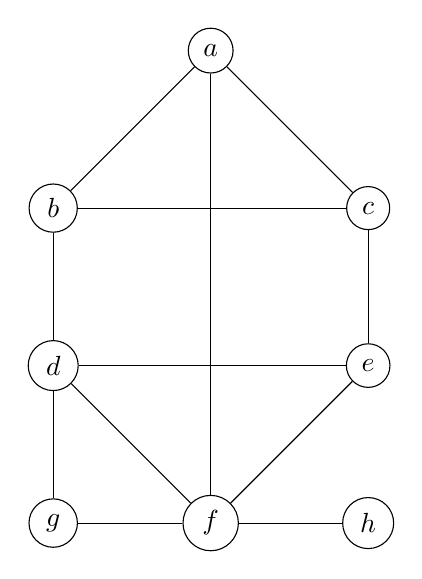
\begin{tikzpicture}
    \node (a) [draw,circle] at (2,6) {\(a\)};
    \node (b) [draw,circle] at (0,4) {\(b\)};
    \node (c) [draw,circle] at (4,4) {\(c\)};
    \node (d) [draw,circle] at (0,2) {\(d\)};
    \node (e) [draw,circle] at (4,2) {\(e\)};
    \node (f) [draw,circle] at (2,0) {\(f\)};
    \node (g) [draw,circle] at (0,0) {\(g\)};
    \node (h) [draw,circle] at (4,0) {\(h\)};
    \draw (a) to (b);
    \draw (a) to (c);
    \draw (a) to (f);
    \draw (b) to (c);
    \draw (b) to (d);
    \draw (c) to (e);
    \draw (d) to (e);
    \draw (d) to (f);
    \draw (d) to (g);
    \draw (e) to (f);
    \draw (f) to (g);
    \draw (f) to (h);
  \end{tikzpicture}
  \caption{An example graph.}
  \label{fig:example}
\end{figure}

The algorithm steps are as follows.  Main routine steps are marked by ``O\#'' and recursive subroutine steps are
marked by ``I\#.''.  Recursive subroutine calls add a call level: ``I\#--\#.''

\begin{enumerate}
\item (O\ref{step:outer:bron}) Use the Bron Kerbosch algorithm to calculate \(k_{min}=3\).

\item (O\ref{step:outer:greedy}) Use the greedy last-first algorithm to calculate \(k_{max}=4\).

\item (O\ref{step:outer:initk}) Initialize \(k=k_{min}=3\).

\item (O\ref{step:outer:match}) \(k=3\ne4=k_{max}\), so continue.

\item (O\ref{step:outer:call}) Call the subroutine with \(G\) and \(k=3\).

\item (I\ref{step:sub:check}) \(n=8\nleq3=k\), so continue.

\item (I\ref{step:sub:dencalc}) Calculate the maximum edge threshold for \(n=8\) and \(k=3\):
  \[a=\frac{n^2(k-1)}{2k}=\frac{8^2(3-1)}{2\cdot3}\approx21.3\]

\item (I\ref{step:sub:density}) \(m=12\ngtr21.3=a\), so continue.

\item (I\ref{step:sub:smallcalc}) \(\deg(g)=2<3\) and \(\deg(h)=1<3\), so set \(X=\set{g,h}\).

\item (I\ref{step:sub:small}) \(X\ne\emptyset\), so replace \(G\) with \(G-X\).  The result is shown in
  \figurename~\ref{fig:removegh}.  Now \(n=6\) and \(m=9\).

  \begin{figure}[H]
    \centering
    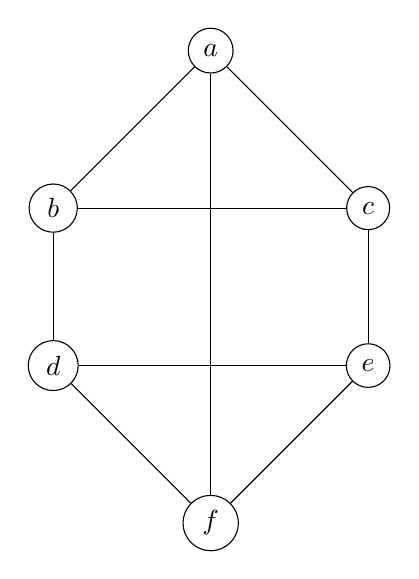
\begin{tikzpicture}
      \node (a) [draw,circle] at (2,6) {\(a\)};
      \node (b) [draw,circle] at (0,4) {\(b\)};
      \node (c) [draw,circle] at (4,4) {\(c\)};
      \node (d) [draw,circle] at (0,2) {\(d\)};
      \node (e) [draw,circle] at (4,2) {\(e\)};
      \node (f) [draw,circle] at (2,0) {\(f\)};
      \draw (a) to (b);
      \draw (a) to (c);
      \draw (a) to (f);
      \draw (b) to (c);
      \draw (b) to (d);
      \draw (c) to (e);
      \draw (d) to (e);
      \draw (d) to (f);
      \draw (e) to (f);
    \end{tikzpicture}
    \caption{Step: \(G-\set{g,h}\).}
    \label{fig:removegh}
  \end{figure}

\item (I\ref{step:sub:check}) \(n=6\nleq3=k\), so continue.

\item (I\ref{step:sub:dencalc}) Calculate the maximum edge threshold for \(n=6\) and \(k=3\):
  \[a=\frac{n^2(k-1)}{2k}=\frac{6^2(3-1)}{2\cdot3}=12\]

\item (I\ref{step:sub:density}) \(m=12\ngtr12=a\), so continue.

\item (I\ref{step:sub:smallcalc}) \(\dmin(G)=3\ge3=k\), so set \(X=\emptyset\).

\item (I\ref{step:sub:small}) \(X=\emptyset\), so continue.

\item (I\ref{step:sub:common}) Calculate the number of common neighbors, looking for any subsets.  The results are
  shown in \tablename~\ref{tab:common}.

  \begin{table}[H]
    \centering
    \caption{Calculating Common Neighbors}
    \label{tab:common}
    \begin{tabular}{|c|c|c|c|c|}
      \hline
      \(u\) & \(v\) & \(\abs{N(u)\cap N(v)}\) & subset? & adjacent? \\
      \hline
      \(a\) & \(b\) & 1 & N & Y \\
      \hline
      \(a\) & \(c\) & 1 & N & Y \\
      \hline
      \(a\) & \(d\) & 2 & N & N \\
      \hline
      \(a\) & \(e\) & 2 & N & N \\
      \hline
      \(a\) & \(f\) & 0 & N & Y \\
      \hline
      \(b\) & \(c\) & 1 & N & Y \\
      \hline
      \(b\) & \(d\) & 0 & N & Y \\
      \hline
      \(b\) & \(e\) & 2 & N & N \\
      \hline
      \(b\) & \(f\) & 2 & N & N \\
      \hline
      \(c\) & \(d\) & 2 & N & N \\
      \hline
      \(c\) & \(e\) & 0 & N & Y \\
      \hline
      \(c\) & \(f\) & 2 & N & N \\
      \hline
      \(d\) & \(e\) & 1 & N & Y \\
      \hline
      \(d\) & \(f\) & 1 & N & Y \\
      \hline
      \(e\) & \(f\) & 1 & N & Y \\
      \hline
    \end{tabular}
  \end{table}

\item (I\ref{step:sub:subset}) There are no \(u,v\in V(G)\) such that \(N(u)\subseteq N(v)\), so continue.

\item (I\ref{step:sub:select}) From \tablename~\ref{tab:common}, the minimum number of common neighbors is 0
  (e.g., \(a\) and \(f\)), so set \(b=0\).

\item (I\ref{step:sub:ubcalc}) Calculate the upper bound for minimum number of common neighbors for \(n=6\) and
  \(k=3\):
  \[c=n-2-\frac{n-2}{k-1}=6-2-\frac{6-2}{3-1}=2\]

\item (I\ref{step:sub:ubcheck}) \(b=0\ngtr2=c\), so conclude that \(G\) may be \colorable{3} and continue.

\item (I\ref{step:sub:select2}) Based on the results in \tablename~\ref{tab:common}, all of the nonadjacent
  vertices share two common neighbors, so select \(a\) and \(d\).

\item (I\ref{step:sub:call1}) Recursively call the subroutine with \(G\cdot ad\), as shown in
  \figurename~\ref{fig:contractad}.  Now, \(n=5\) and \(m=7\).

  \begin{figure}[H]
    \centering
    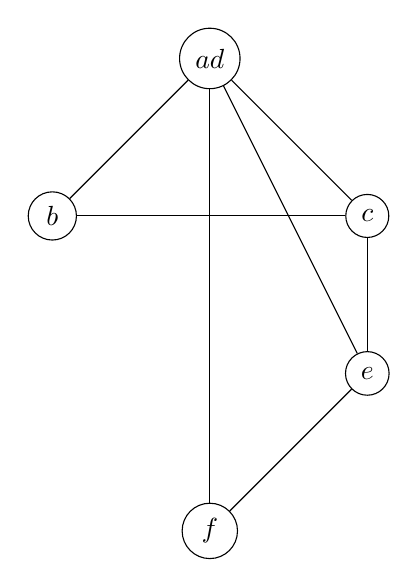
\begin{tikzpicture}
      \node (ad) [draw,circle] at (2,6) {\(ad\)};
      \node (b) [draw,circle] at (0,4) {\(b\)};
      \node (c) [draw,circle] at (4,4) {\(c\)};
      \node (e) [draw,circle] at (4,2) {\(e\)};
      \node (f) [draw,circle] at (2,0) {\(f\)};
      \draw (ad) to (b);
      \draw (ad) to (c);
      \draw (ad) to (f);
      \draw (b) to (c);
      \draw (c) to (e);
      \draw (ad) to (e);
      \draw (e) to (f);
    \end{tikzpicture}
    \caption{Step: \(G\cdot ad\).}
    \label{fig:contractad}
  \end{figure}

\item (I\ref{step:sub:check}-1) \(n=5\nleq3=k\), so continue.

\item (I\ref{step:sub:dencalc}-1) Calculate the maximum edge threshold for \(n=5\) and \(k=3\):
  \[a=\frac{n^2(k-1)}{2k}=\frac{5^2(3-1)}{2\cdot3}\approx8.3\]

\item (I\ref{step:sub:density}-1) \(m=7\ngtr8.3=a\), so conclude that \(G\) may be \colorable{3} and continue.
  
\item (I\ref{step:sub:smallcalc}-1) \(\deg(b)=\deg(f)=2<3=k\), so set \(X=\set{b,f}\).

\item (I1-\ref{step:sub:small}-1) \(X\ne\emptyset\), so replace \(G\) with \(G-X\).  The result is shown in Figure
  \ref{fig:removecf}.  Now \(n=3\) and \(m=3\).

  \begin{figure}[H]
    \centering
    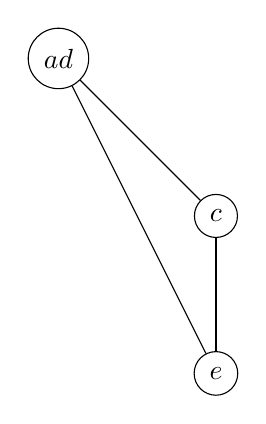
\begin{tikzpicture}
      \node (ad) [draw,circle] at (2,6) {\(ad\)};
      \node (c) [draw,circle] at (4,4) {\(c\)};
      \node (e) [draw,circle] at (4,2) {\(e\)};
      \draw (ad) to (c);
      \draw (c) to (e);
      \draw (e) to (ad);
    \end{tikzpicture}
    \caption{Step: \(G-\set{b,f}\)}
    \label{fig:removecf}
  \end{figure}

\item (I\ref{step:sub:check}-1) \(n=3\le3=k\), so conclude that the \(G\) of \figurename~\ref{fig:removecf} is
  \colorable{3} and return true.

\item (I\ref{step:sub:result1}) The recursive call returned true, so conclude that the \(G\) of
  \figurename~\ref{fig:removecf} is \colorable{3} and return true.

\item (O\ref{step:outer:result})\label{step:last} The recursive subroutine returned true, so conclude that the \(G\)
  is \chromatic{3} and return \(\X(G)=3\).
\end{enumerate}

Thus, the algorithm determines that the example \(G\) of Figure \ref{fig:example} is \chromatic{3} in
\ref{step:last} steps.  In order to determine a \chromatic{3} coloring for \(G\), first construct a set \(C\) of
three colors:
\[C=\set{\text{\textcolor{green}{green}},\text{\textcolor{blue}{blue}},\text{\textcolor{red}{red}}}\]
Next, follow the algorithm's modification steps in reverse order and color the corresponding vertices accordingly.
The steps are as follows:

\begin{enumerate}
\item First, color the vertices that are present in the final simplified graph.  Assign each vertex its own color,
  except assign contracted vertices the same color.  This is shown in \figurename~\ref{fig:cstart}.
  
  \begin{figure}[H]
    \centering
    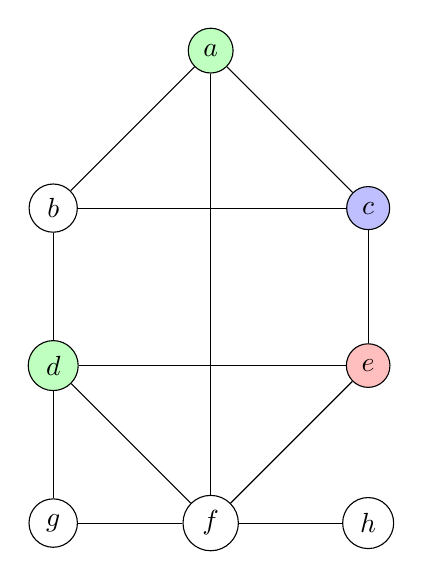
\begin{tikzpicture}
      \colorlet{c1}{green!25!white}
      \colorlet{c2}{blue!25!white}
      \colorlet{c3}{red!25!white}
      \node [fill=c1] (a) [draw,circle] at (2,6) {\(a\)};
      \node (b) [draw,circle] at (0,4) {\(b\)};
      \node [fill=c2] (c) [draw,circle] at (4,4) {\(c\)};
      \node [fill=c1] (d) [draw,circle] at (0,2) {\(d\)};
      \node [fill=c3] (e) [draw,circle] at (4,2) {\(e\)};
      \node (f) [draw,circle] at (2,0) {\(f\)};
      \node (g) [draw,circle] at (0,0) {\(g\)};
      \node (h) [draw,circle] at (4,0) {\(h\)};
      \draw (a) to (b);
      \draw (a) to (c);
      \draw (a) to (f);
      \draw (b) to (c);
      \draw (b) to (d);
      \draw (c) to (e);
      \draw (d) to (e);
      \draw (d) to (f);
      \draw (d) to (g);
      \draw (e) to (f);
      \draw (f) to (g);
      \draw (f) to (h);
    \end{tikzpicture}
    \caption{Initial coloring.}
    \label{fig:cstart}
  \end{figure}

\item The last modification was the removal of vertices \(b\) and \(f\).  Note that color selection needs to honor
  the vertices already colored.  This is shown in \figurename~\ref{fig:colorbf}.

  \begin{figure}[H]
    \centering
    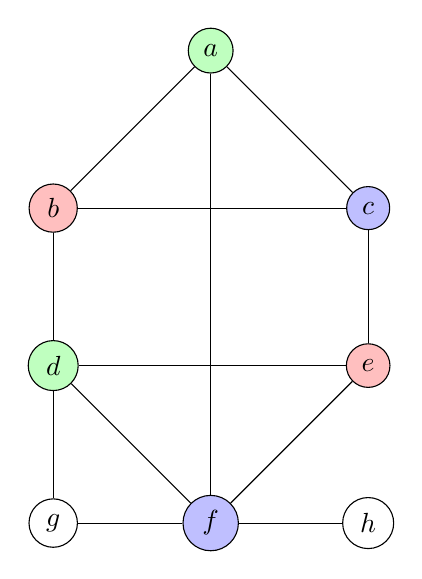
\begin{tikzpicture}
      \colorlet{c1}{green!25!white}
      \colorlet{c2}{blue!25!white}
      \colorlet{c3}{red!25!white}
      \node [fill=c1] (a) [draw,circle] at (2,6) {\(a\)};
      \node [fill=c3] (b) [draw,circle] at (0,4) {\(b\)};
      \node [fill=c2] (c) [draw,circle] at (4,4) {\(c\)};
      \node [fill=c1] (d) [draw,circle] at (0,2) {\(d\)};
      \node [fill=c3] (e) [draw,circle] at (4,2) {\(e\)};
      \node [fill=c2] (f) [draw,circle] at (2,0) {\(f\)};
      \node (g) [draw,circle] at (0,0) {\(g\)};
      \node (h) [draw,circle] at (4,0) {\(h\)};
      \draw (a) to (b);
      \draw (a) to (c);
      \draw (a) to (f);
      \draw (b) to (c);
      \draw (b) to (d);
      \draw (c) to (e);
      \draw (d) to (e);
      \draw (d) to (f);
      \draw (d) to (g);
      \draw (e) to (f);
      \draw (f) to (g);
      \draw (f) to (h);
    \end{tikzpicture}
    \caption{Coloring \(b\) and \(f\).}
    \label{fig:colorbf}
  \end{figure}

\item Finally, color the first removed vertices \(g\) and \(h\) with any appropriate color.  The final result is
  shown in \figurename~\ref{fig:cfinal}.

  \begin{figure}[H]
    \centering
    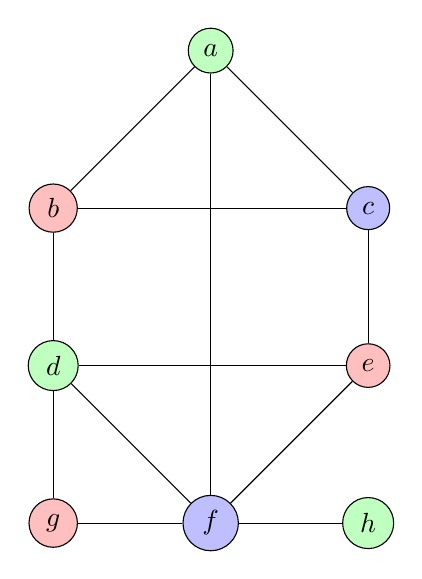
\begin{tikzpicture}
      \colorlet{c1}{green!25!white}
      \colorlet{c2}{blue!25!white}
      \colorlet{c3}{red!25!white}
      \node [fill=c1] (a) [draw,circle] at (2,6) {\(a\)};
      \node [fill=c3] (b) [draw,circle] at (0,4) {\(b\)};
      \node [fill=c2] (c) [draw,circle] at (4,4) {\(c\)};
      \node [fill=c1] (d) [draw,circle] at (0,2) {\(d\)};
      \node [fill=c3] (e) [draw,circle] at (4,2) {\(e\)};
      \node [fill=c2] (f) [draw,circle] at (2,0) {\(f\)};
      \node [fill=c3] (g) [draw,circle] at (0,0) {\(g\)};
      \node [fill=c1] (h) [draw,circle] at (4,0) {\(h\)};
      \draw (a) to (b);
      \draw (a) to (c);
      \draw (a) to (f);
      \draw (b) to (c);
      \draw (b) to (d);
      \draw (c) to (e);
      \draw (d) to (e);
      \draw (d) to (f);
      \draw (d) to (g);
      \draw (e) to (f);
      \draw (f) to (g);
      \draw (f) to (h);
    \end{tikzpicture}
    \caption{Final chromatic coloring.}
    \label{fig:cfinal}
  \end{figure}

\end{enumerate}

At first glance, one might wonder what advantage this method of coloring has over other sequential methods.  The
difference is that the other sequential methods only have knowledge about what has already been colored, whereas
this method uses assumptions that are made during the simplifications and recursive calls on the entire graph.
Thus, the sequential algorithms are heuristic, but this method selects a particular workable coloring path through
the resulting Zykov tree.
